\section{Results}

The possible implementation of the ClaRyS Compton camera as a monitoring system for ion beam therapy has been tested. The detection efficiency of the camera has been measured with the irradiation with point-like gamma sources set in different positions with respect to the center of the camera. A PMMA cylindrical phantom has been simulated and exposed to proton and carbon beams at increasing intensities for an analysis of the prompt gamma detection environment (background, random coincidence contamination). The camera precision in the identification of the fall-off of the prompt gamma emission profile has been investigated. For this purpose, the comparison of two different reconstruction methods (line-cone analytical reconstruction and MLEM iterative algorithm) is presented. In the following sections we show the obtained results. 


\subsection{Absolute detection efficiency}
\label{Results::efficiency}

Figure~\ref{fig::efficiency_study} shows the absolute gamma detection efficiency as a function of the gamma source position with respect to the center of the camera in the transverse plane. On the left side, we show the results achieved with an ideal detector, while on the right side realistic energy cuts are applied on each detector section: the lower energy limit  has been set to 50~keV for the scatterer and 100~keV for the absorber.

\begin{figure} [!hbtp]	
\centering
\subfloat[]{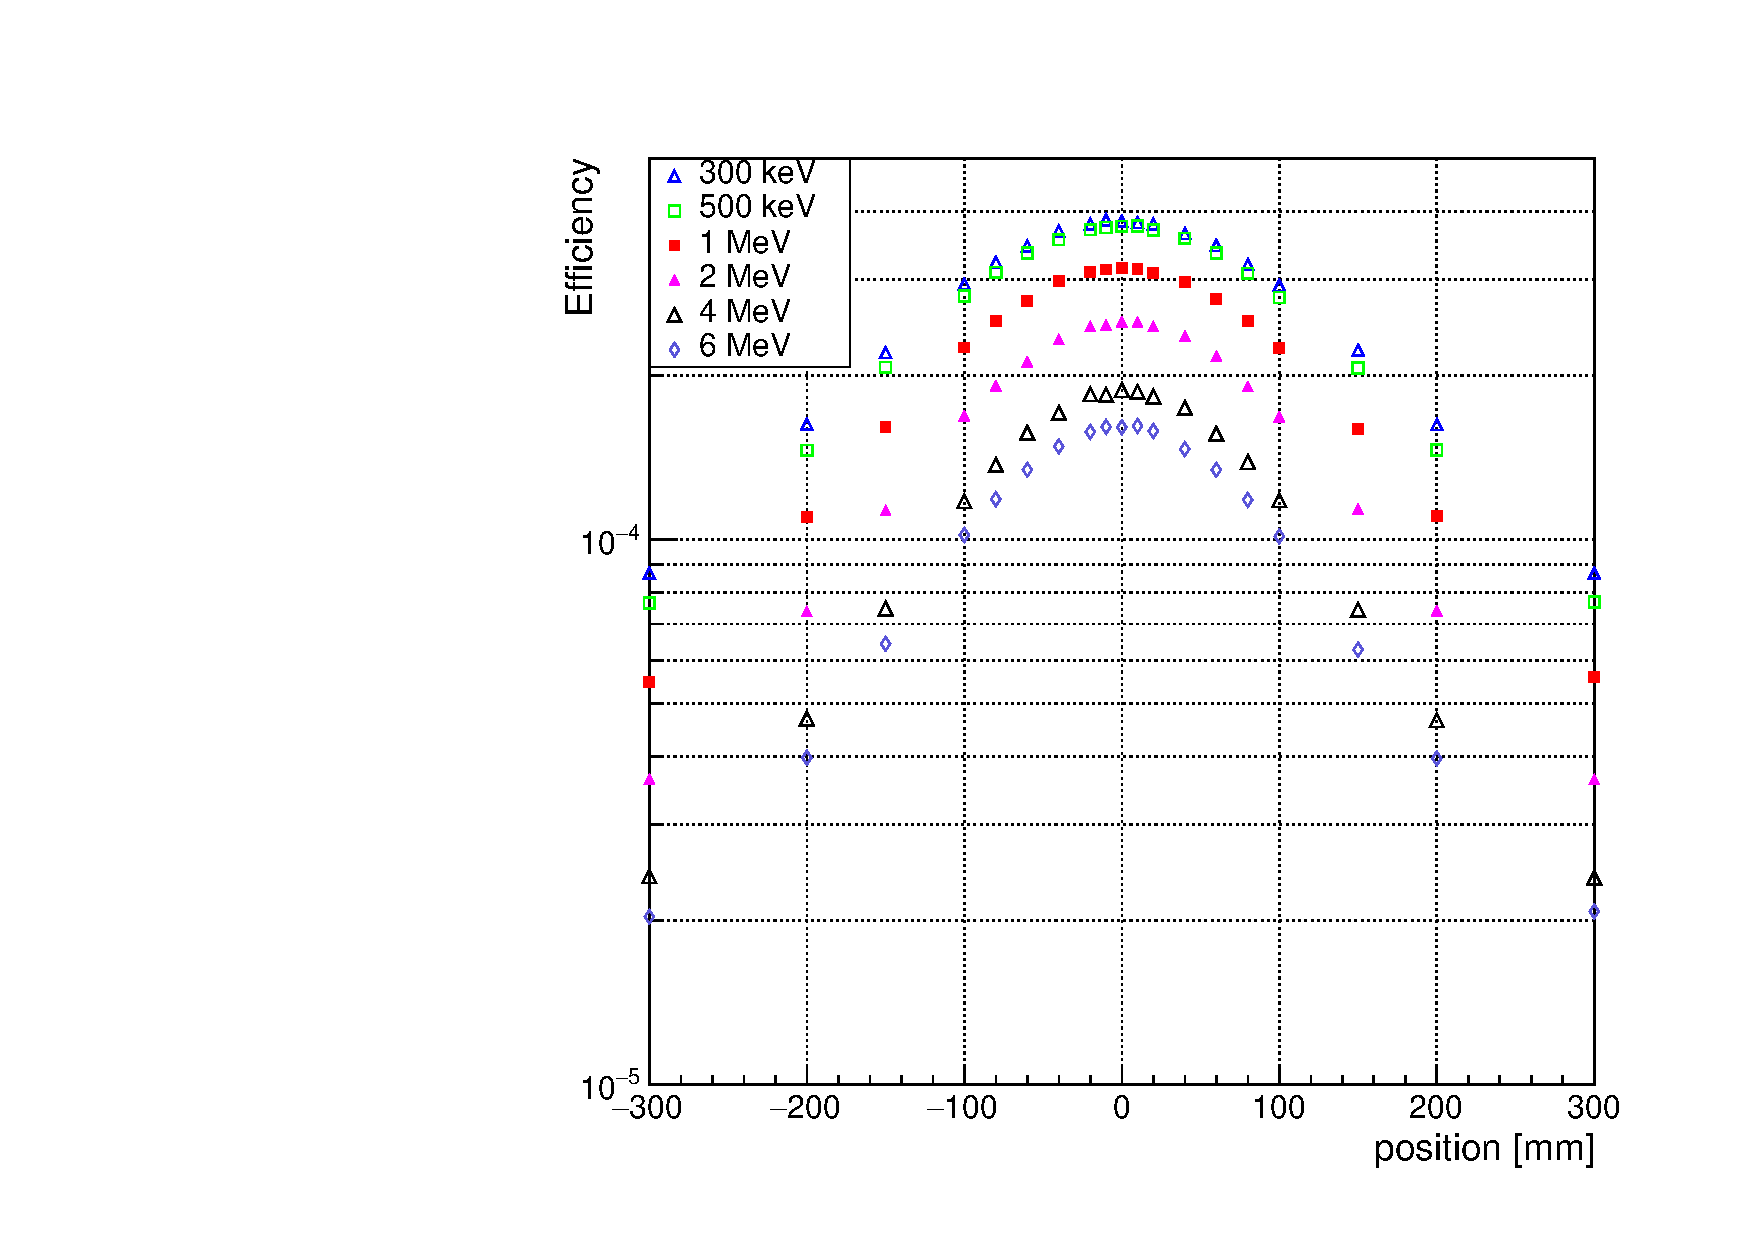
\includegraphics[width=0.5\textwidth]{./Figure/EffVSpos.pdf}}
\subfloat[]{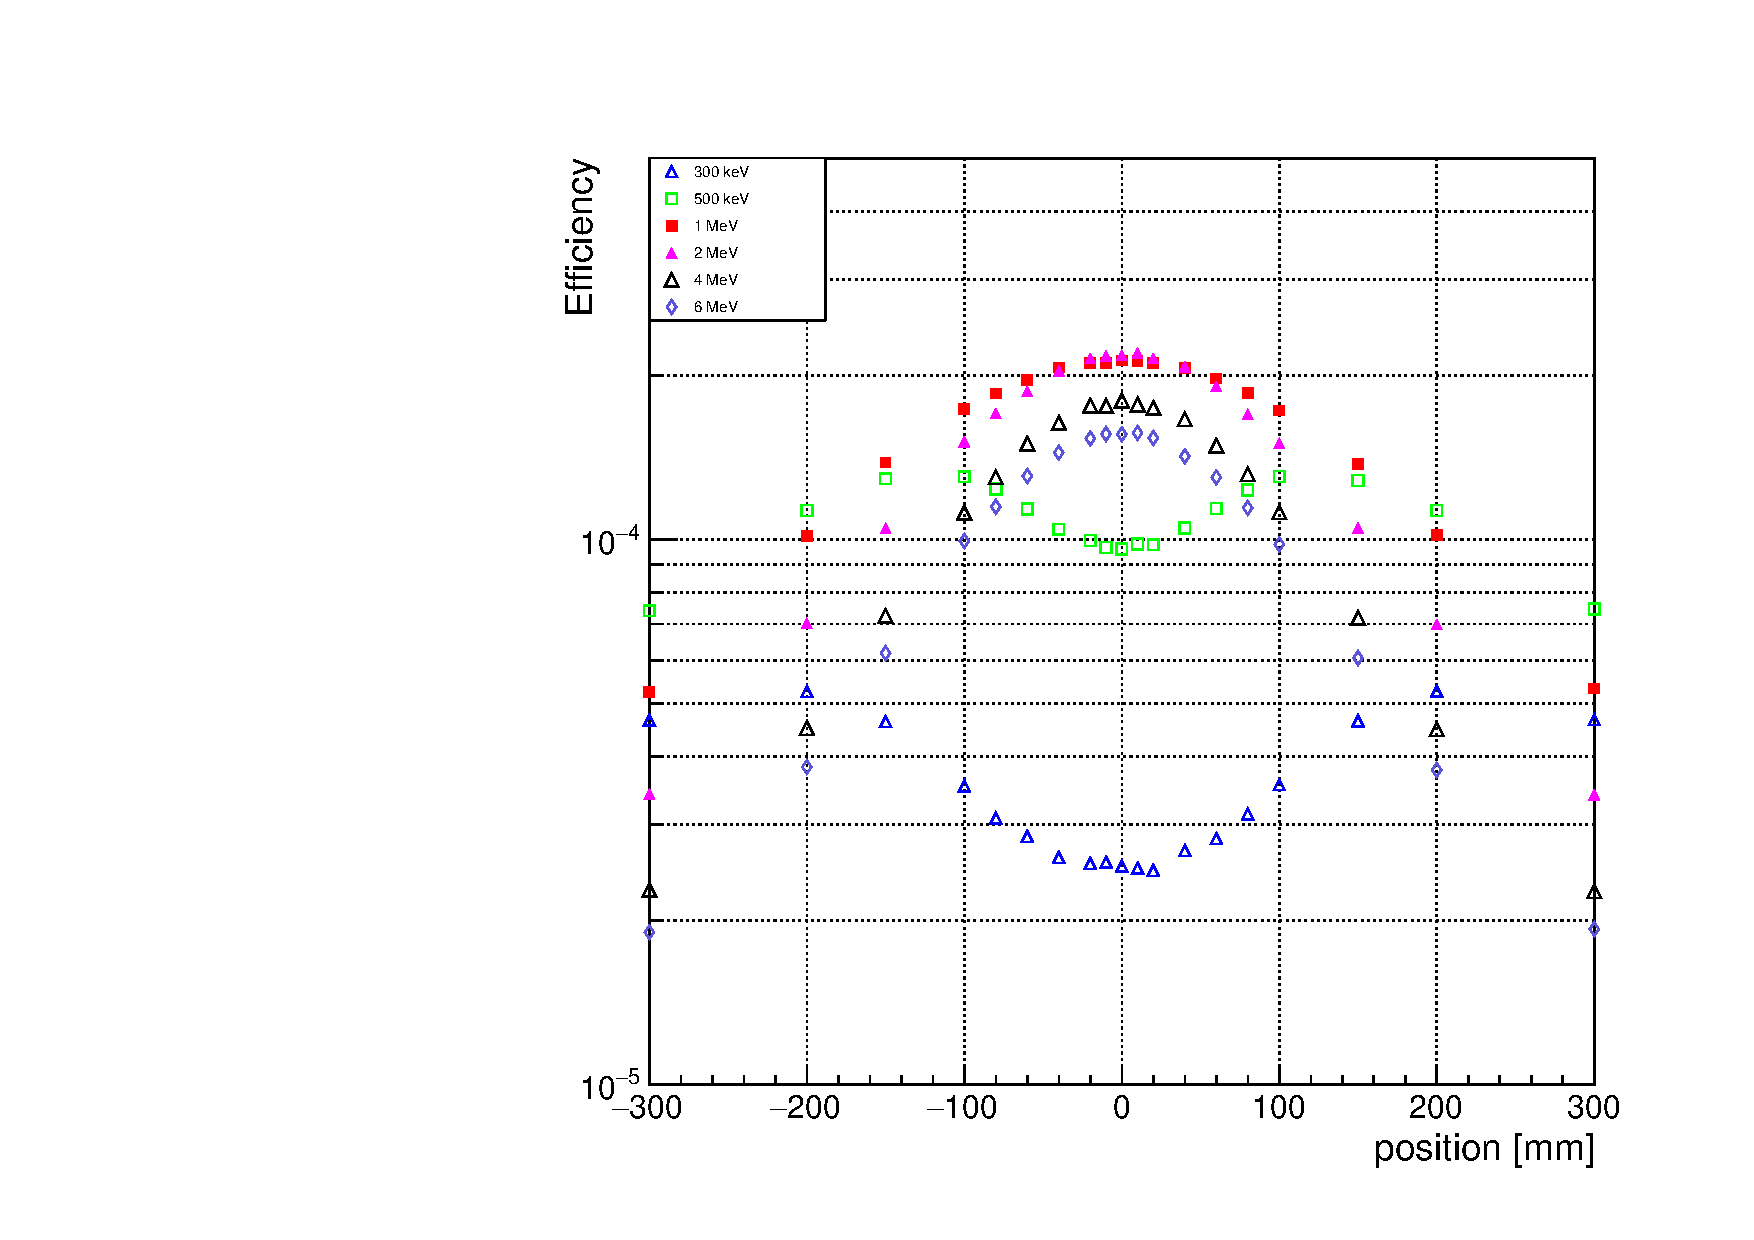
\includegraphics[width=0.5\textwidth]{./Figure/EffVSpos_withCut.pdf}}
\caption{Absolute Compton camera efficiency as a function of the gamma source position for different gamma energies, in the range between 300~keV to 6~MeV. The left side shows the camera efficiency with no data selection. In the right side, detection energy thresholds are applied: the lower energy thresholds are set to 
50~keV for the scatterer and 100~keV for the absorber, to reproduce a realistic scenario. These values can change for the final configuration, according to the detector energy resolutions achieved.}
\label{fig::efficiency_study}
\end{figure}

As expected according to the interaction probability energy dependency, the efficiency is higher for low gamma energies, and it lies in the range $4\times10^{-4}$ at 300~keV and $1.5\times10^{-4}$ at 6~MeV (figure \ref{fig::efficiency_study}). Moreover, it can be noticed how the efficiency quickly drops as the point source is shifted away from the camera center: this effect is more important for high energies, for which the incident gamma is less deflected in the scatterer for the same energy deposited compared to a low energy gamma (see equation~\ref{Compton_equation}).\\ 
Figure~\ref{fig::efficiency_study}(b) shows the effect of realistic camera detection thresholds as opposed to ideal detection. The gamma detection efficiency drops of a factor ranging from about 1.25 to more than an order of magnitude for the central detection area for energies in the range 300~keV - 2~MeV respectively. The effect is reduced by the distance of the source from the center of the camera. Negligible effects are detected for positions with a distance greater than 200~mm from the center of the camera, and for any distance at energies above 2~MeV, while the efficiency is reduced for low energy gammas in the central area of the camera. 

\subsection{Rate of random coincidences}
\label{Results::beamInt}
 
In figure~\ref{fig:coincidences}, the different components of the signal resulting from the PMMA exposure to proton and carbon beams are shown as a function of the beam intensity. The true coincidences represent scatterer-absorber time coincidences generated by the same gamma ray. All the other coincidence types compose the background. The collected data sets are reported with and without the applied time-of-flight discrimination, mainly employed for neutron rejection, as mentioned in section~\ref{MatMeth::TOF_Ecut}.


\begin{figure} [!h]
  \subfloat[]{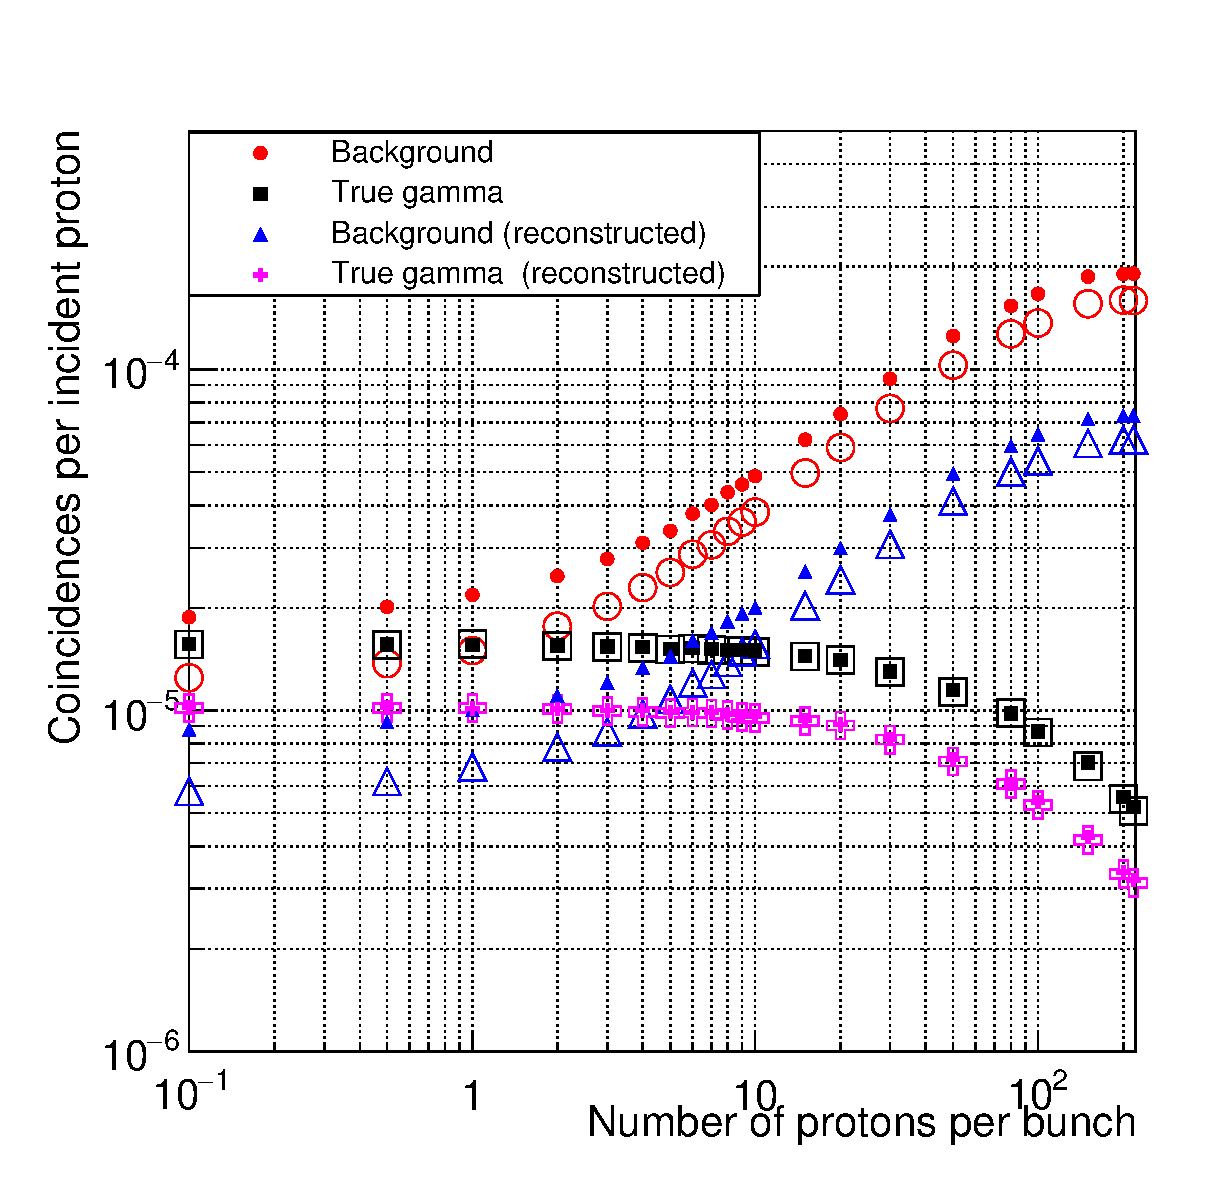
\includegraphics[width=0.5\textwidth]{./Figure/2017_06_28_Taux_coincidences_variation_protons_New_design_4EntreesLegend_LogXLogY.eps}}
  \subfloat[]{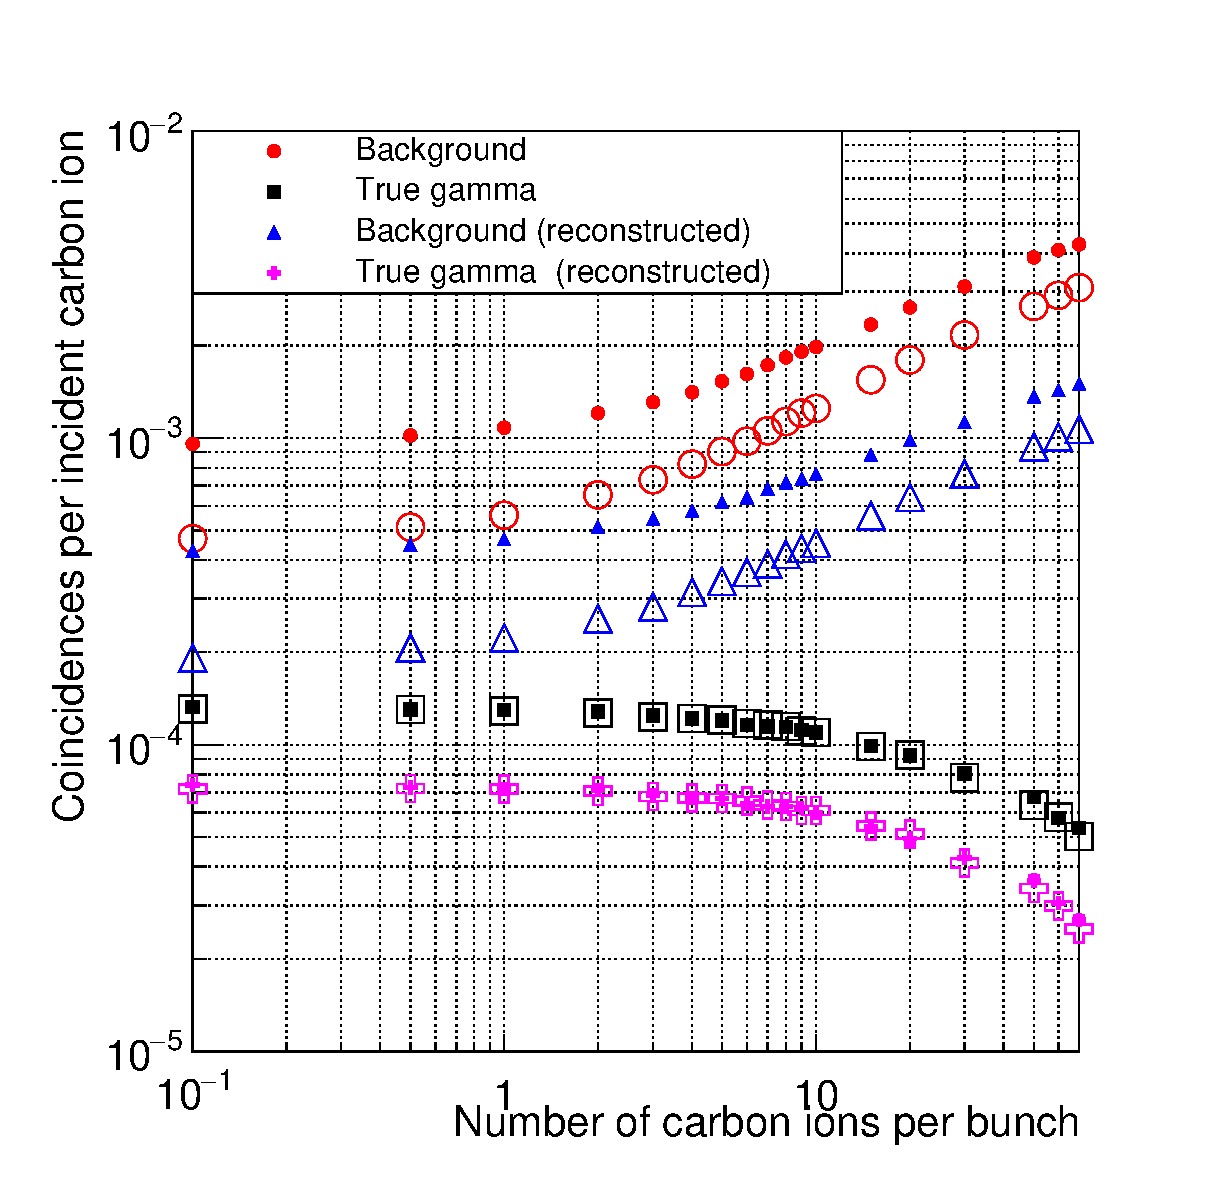
\includegraphics[width=0.5\textwidth]{./Figure/2017_06_28_Taux_coincidences_variation_carbonIons_New_design_4EntreesLegend_LogXLogY.eps}}
  \caption{Coincidences yield for protons (left) and carbon ions (right) as a function of the beam intensity. The intensity is reported as number of incident particles per bunch. The filled markers correspond to the collected data without time-of-flight discrimination, while this cut is applied to the data reported with empty markers. Moreover, the yields are given before and after the profile reconstruction with the line-cone algorithm.}
  \label{fig:coincidences}
\end{figure}

In figure~\ref{fig:coincidences}(a) and (b) the amount of true gamma coincidences and background events are reported before and after reconstruction via line-cone algorithm as a function of the beam intensity for proton (a) and carbon ion (b) beams. In addition to this, for each curve realized with the complete collected data set, the related one realized after time-of-flight selection of events is sketched. All the curves have been normalized to the number of incident ions.

The amount of background events (mainly random coincidences) increases with the increasing beam intensity: a factor of about 30 with respect to true gamma events is obtained for proton beams at  the intensity of 200 protons per bunch with no event selection, while a factor more than two times higher is reported for carbon ions in the same conditions. The time-of-flight selection can slightly improve the signal -over-noise ratio by reducing the amount of background events. The amount of true gamma events and background events becomes similar at the intensity of about 1 proton per bunch.


\subsection{Camera precision}
\label{Results::precision_reconstruction}
Given the results presented in the previous section, the camera precision in the fall-off identification is investigated with proton beams at reduced intensities.
%The simulation setup shown in figure~\ref{fig:fig_setup_CC_simulation_Hadronth} has been implemented to test the line-cone analytic reconstruction method and compare it to the iterative LM-MLEM algorithm~\cite{maxim_filtered_2014,hilaire_compton_2014}. 
A single data set has been collected, corresponding to the irradiation of the PMMA phantom with a proton 160~MeV monoenergetic beam, with a reduced intensity of 1 proton per bunch. A total of $10^{10}$ protons has been simulated to define the reference Bragg peak, and then different sub-data sets have been extracted for the precision estimate at different statistics, as explained in section~\ref{MatMeth:precision}. 

The high statistics profile reconstructed via line-cone algorithm is shown in figure~\ref{fig:fig_Results_Estimation_Camera_Profil_highStat_CC_simulation_Hadronth_LineCone} and via the LM-MLEM reconstruction method in figure~\ref{fig:fig_Results_Estimation_Camera_Profil_highStat_CC_simulation_Hadronth_MLEM}. A NURBS model of a low statistics subset sample ($10^8$ incident protons) is shown in figures~\ref{fig:fig_Estimation_Camera_CC_NURBS_Poisson_LC} for the line cone and~\ref{fig:fig_Estimation_Camera_CC_NURBS_Poisson_MLEM} for the MLEM.
Figures~\ref{fig:fig_Results_Chi2_Distribution_Variation_CC_simulation_Hadronth_LC} and~\ref{fig:fig_Results_Chi2_Distribution_Variation_CC_simulation_Hadronth_MLEM} show the distribution of $\chi^2$ calculated for a low statistic profile at $10^8$ incident protons. The retrieved optimal shift distribution is shown in figure~\ref{fig:fig_Results_Precision_Distribution_Variation_CC_simulation_Hadronth_LC} and~\ref{fig:fig_Results_Precision_Distribution_Variation_CC_simulation_Hadronth_MLEM} for the line-cone and LM-MLEM algorithm respectively, for $10^8$ incident protons as well.
Figure~\ref{fig:comparison} shows the results of the reconstruction of the data set obtained for the selection of 10$^8$ primary protons.


\begin{figure}
  \centering
  \subfloat[\label{fig:fig_Results_Estimation_Camera_Profil_highStat_CC_simulation_Hadronth_LineCone}]{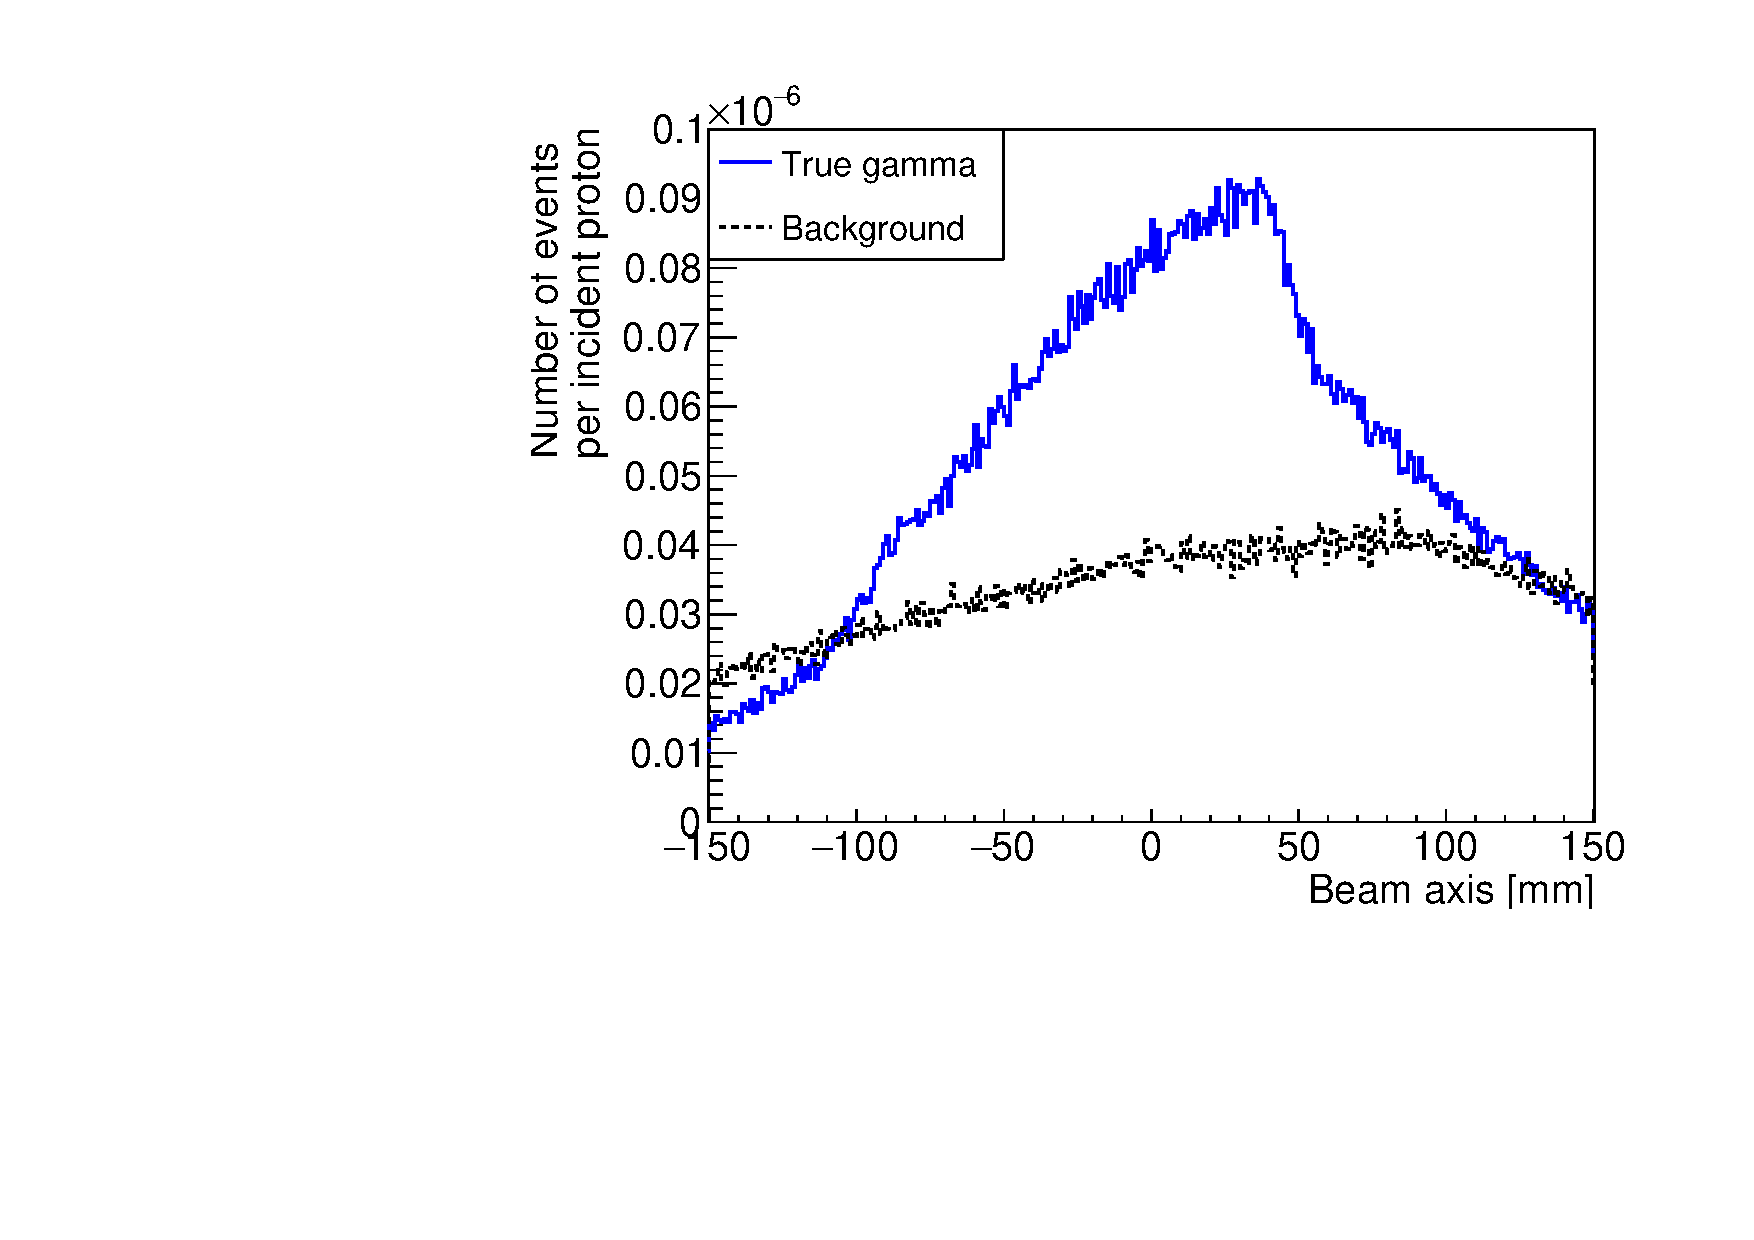
\includegraphics[width=0.48\textwidth]{./Figure/profile_high_stat_linecone_2.pdf}}
  \subfloat[\label{fig:fig_Results_Estimation_Camera_Profil_highStat_CC_simulation_Hadronth_MLEM}]{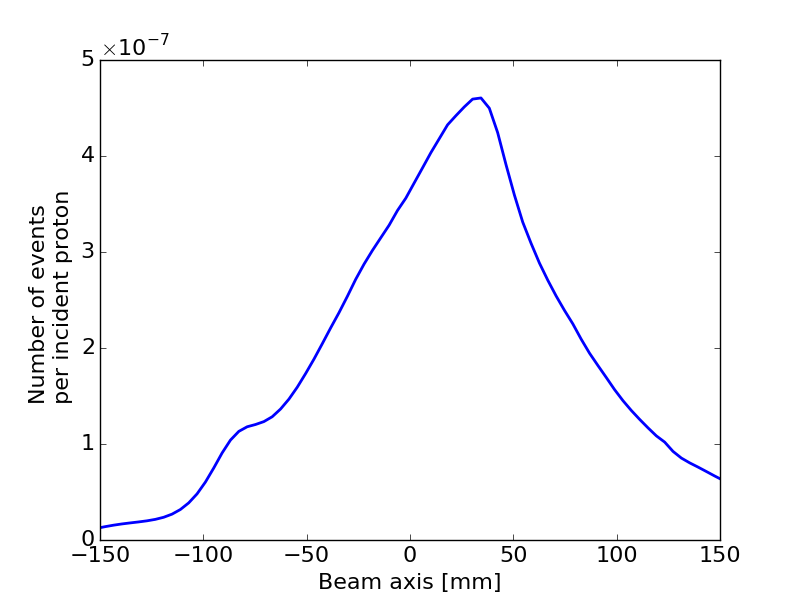
\includegraphics[width=0.48\textwidth]{./Figure/profileY_corr_r15.png}}\\
  % \subfloat[\label{fig:fig_Estimation_Camera_CC_NURBS_Poisson_LC}]{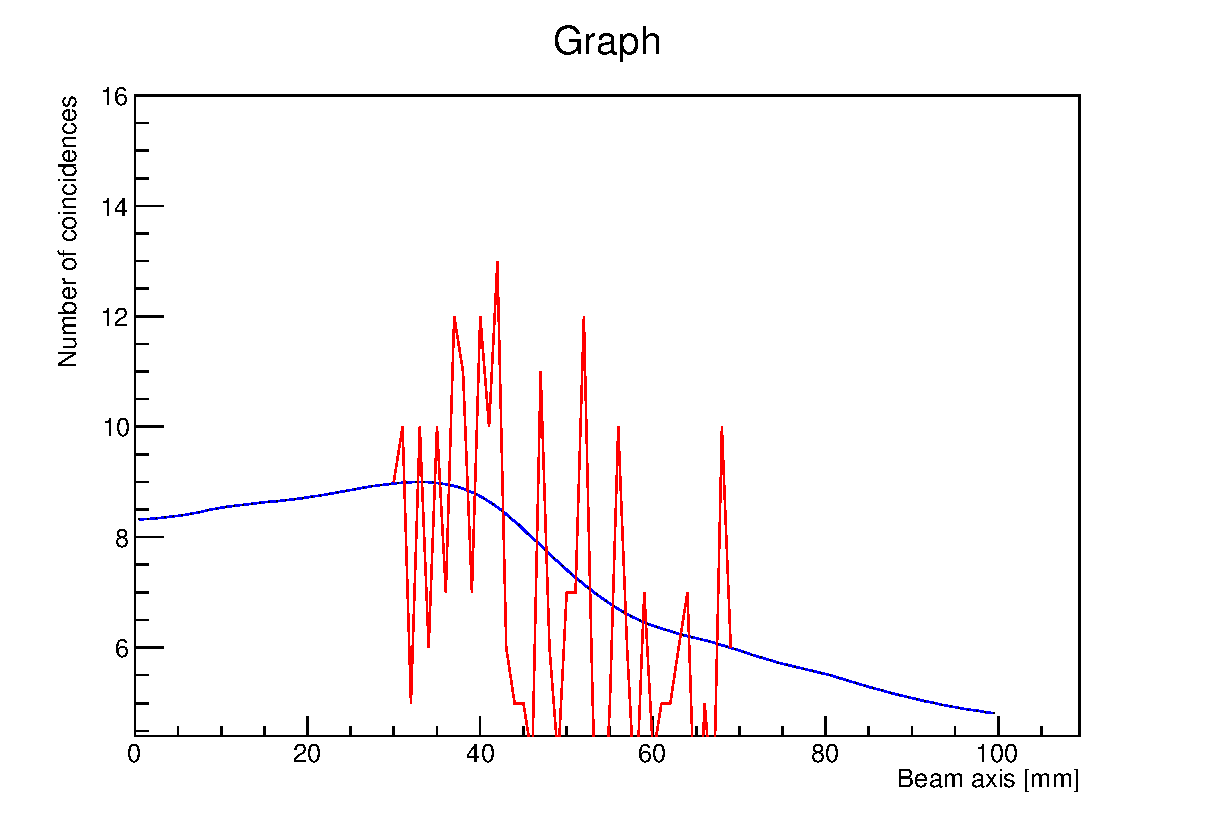
\includegraphics[width=0.33\textwidth]{./Figure/2017-08-02_Poisson_Nurbs_1e8_Article_LC.eps}}
  \subfloat[\label{fig:fig_Estimation_Camera_CC_NURBS_Poisson_LC}]{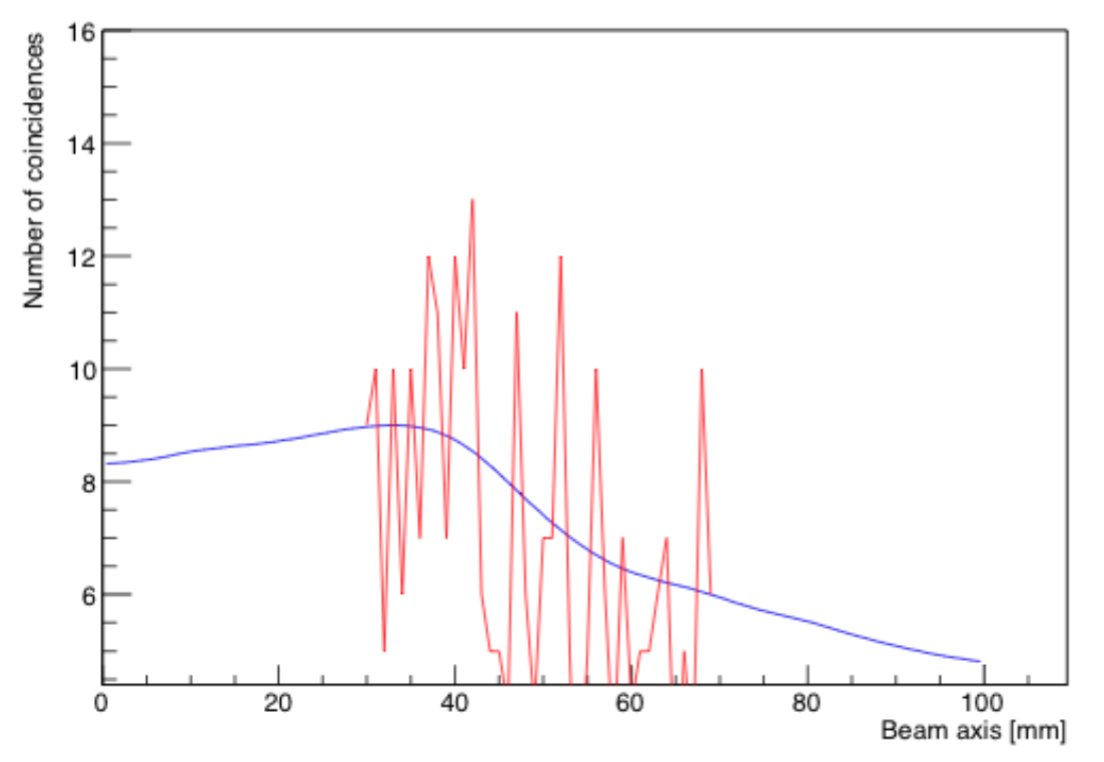
\includegraphics[width=0.48\textwidth]{./Figure/line_cone_NURBS.png}}
  % \subfloat[\label{fig:fig_Estimation_Camera_CC_NURBS_Poisson_MLEM}]{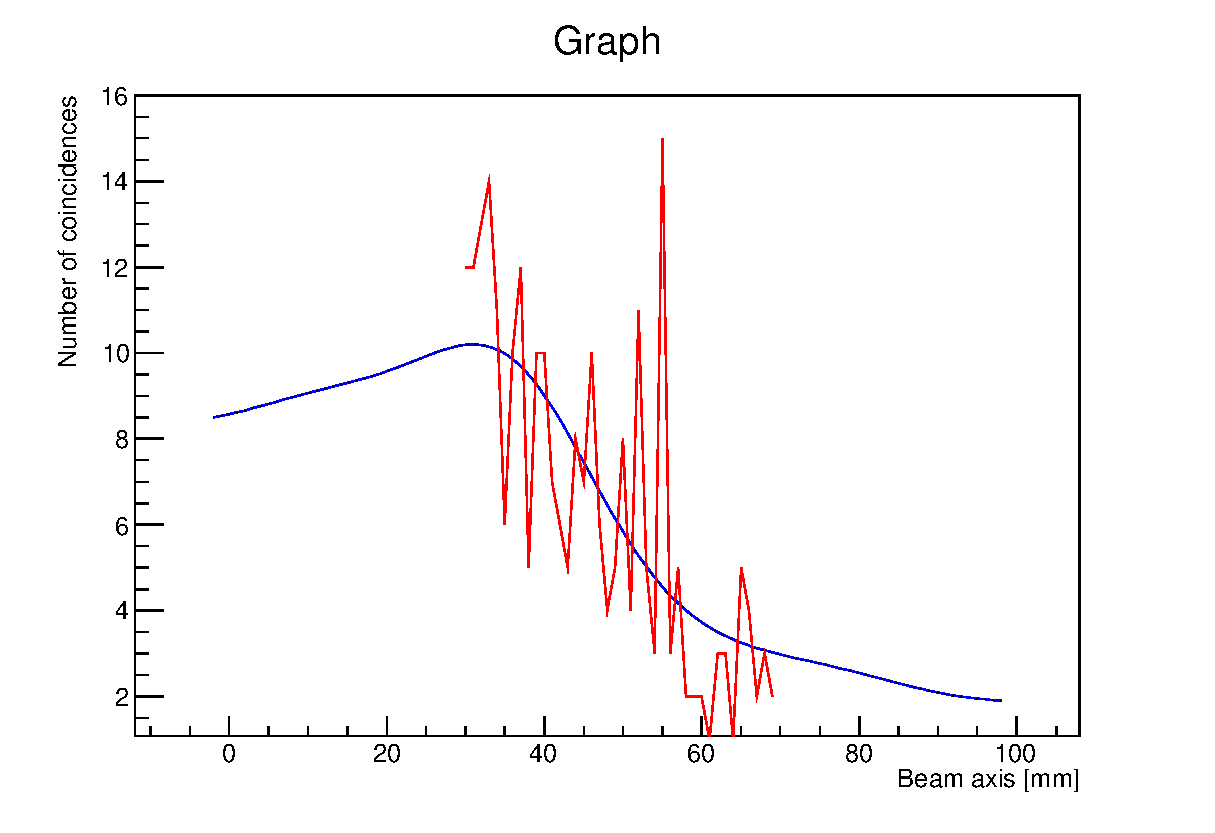
\includegraphics[width=0.33\textwidth]{./Figure/2017-08-02_Nurbs_Poisson_1e8_Article_MLEM.eps}}\\
  \subfloat[\label{fig:fig_Estimation_Camera_CC_NURBS_Poisson_MLEM}]{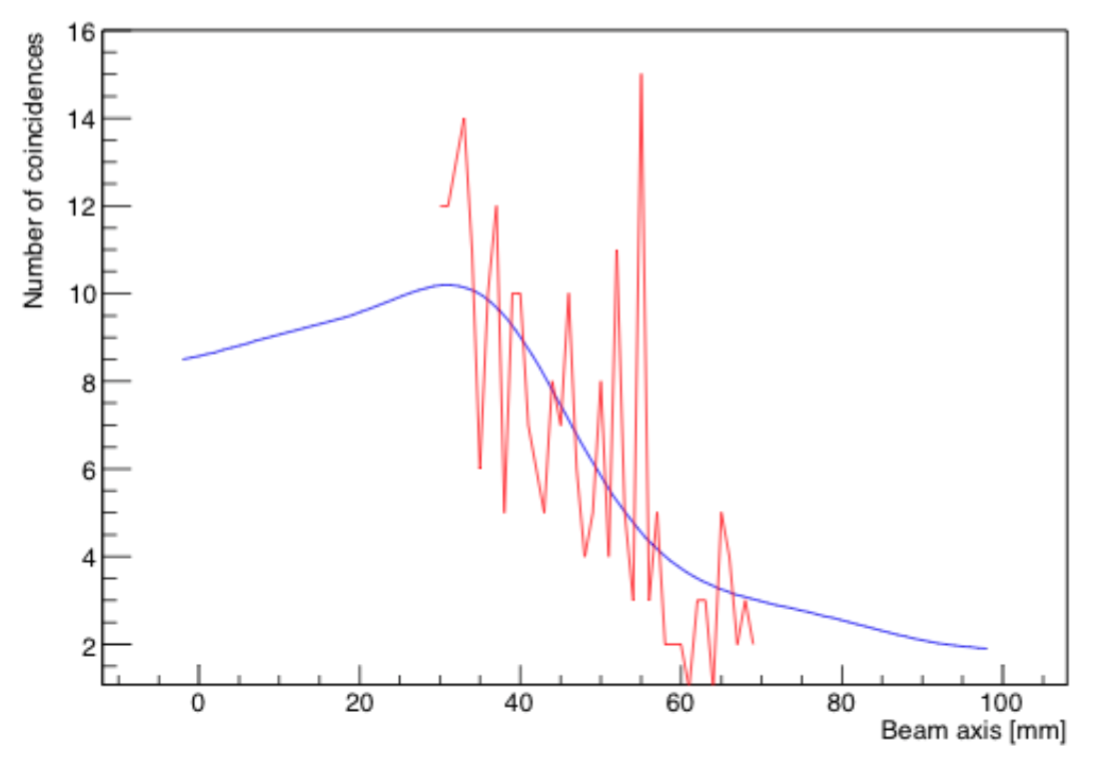
\includegraphics[width=0.48\textwidth]{./Figure/MLEM_NURBS.png}}\\
  \caption{Data processing comparison for the same proton simulation with the line cone algorithm (left column) and the LM-MLEM algorithm (right column). The first row gives the reconstructed profile for $10^{10}$ incident protons. The second row shows the reference curve (blue) and the curve obtained with a $10^8$ incident protons subset.}% at the same statistics of $10^8$ incident protons.}
\end{figure}

\begin{figure}
  \centering
  % \subfloat[\label{fig:fig_Results_Chi2_Distribution_Variation_CC_simulation_Hadronth_LC}]{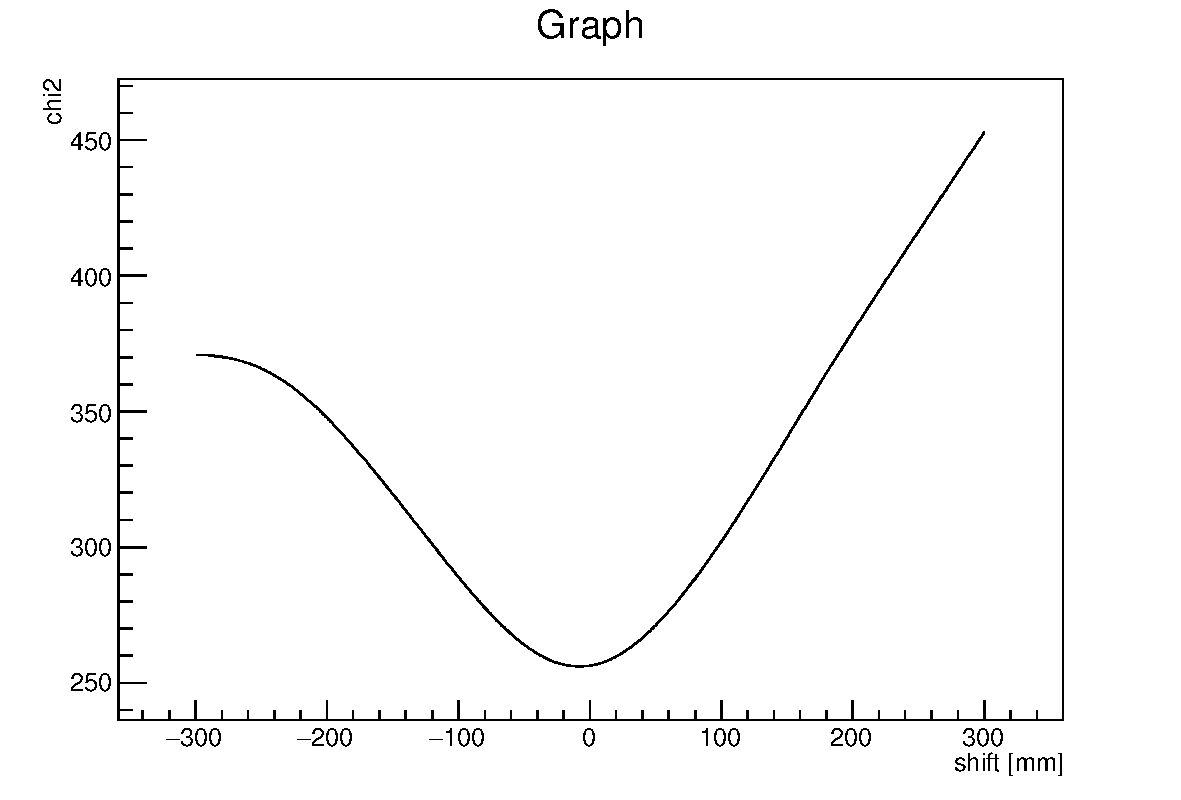
\includegraphics[width=0.33\textwidth]{./Figure/2017-08-02_Distribution_Chi2_1e8_LC.pdf}}
  \subfloat[\label{fig:fig_Results_Chi2_Distribution_Variation_CC_simulation_Hadronth_LC}]{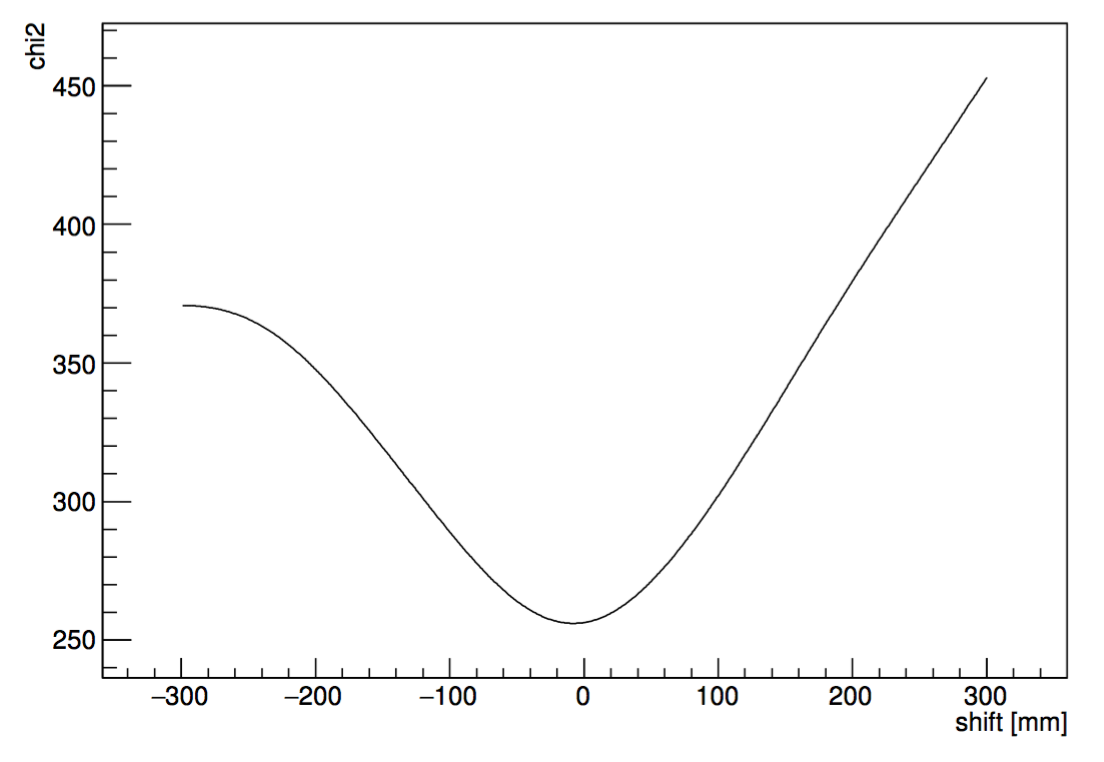
\includegraphics[width=0.48\textwidth]{./Figure/chi2_linecone.png}}
  % \subfloat[\label{fig:fig_Results_Chi2_Distribution_Variation_CC_simulation_Hadronth_MLEM}]{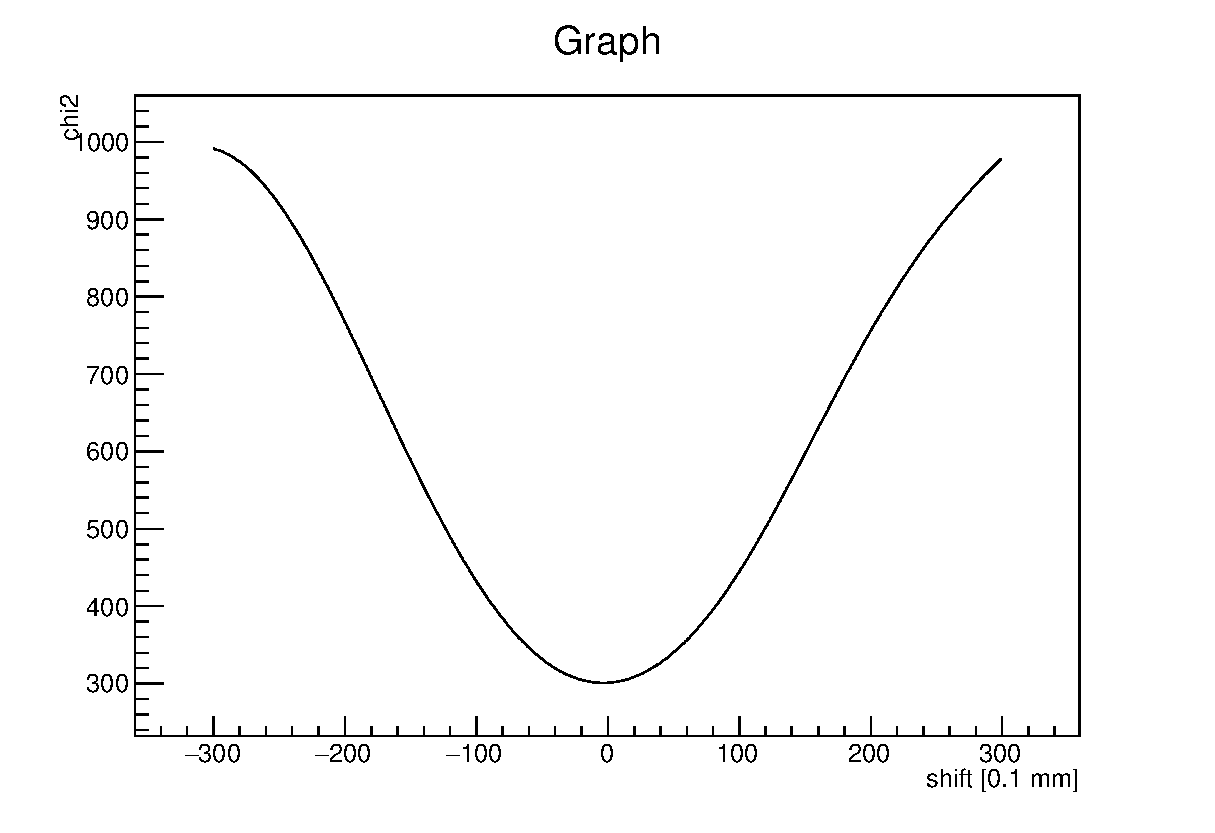
\includegraphics[width=0.33\textwidth]{./Figure/2017-08-02_Distribution_Chi2_Results_binning_1mm_ShiftNurbs0_1mm_1e8_article_MLEM.eps}}\\
  \subfloat[\label{fig:fig_Results_Chi2_Distribution_Variation_CC_simulation_Hadronth_MLEM}]{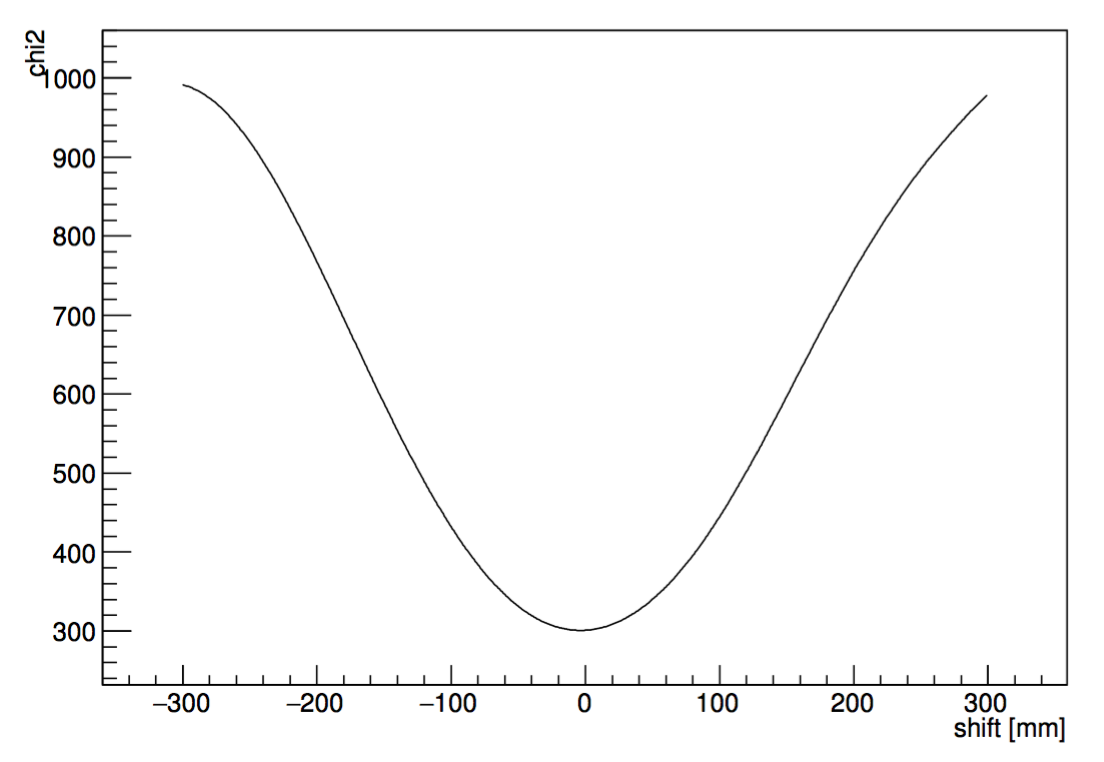
\includegraphics[width=0.48\textwidth]{./Figure/chi2_MLEM.png}}\\
  % \subfloat[\label{fig:fig_Results_Precision_Distribution_Variation_CC_simulation_Hadronth_LC} ]{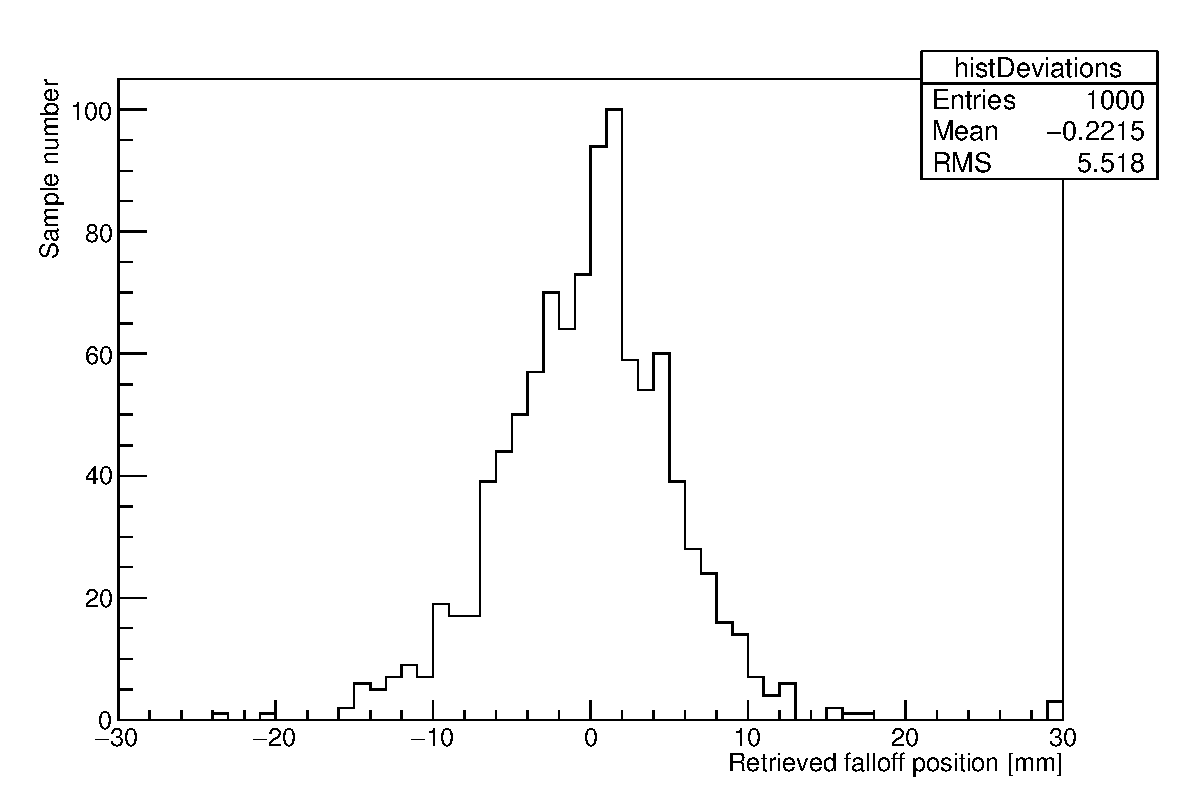
\includegraphics[width=0.33\textwidth]{./Figure/2017-08-02_Distribution_finale_1e8_Article_LC.pdf}}
  \subfloat[\label{fig:fig_Results_Precision_Distribution_Variation_CC_simulation_Hadronth_LC} ]{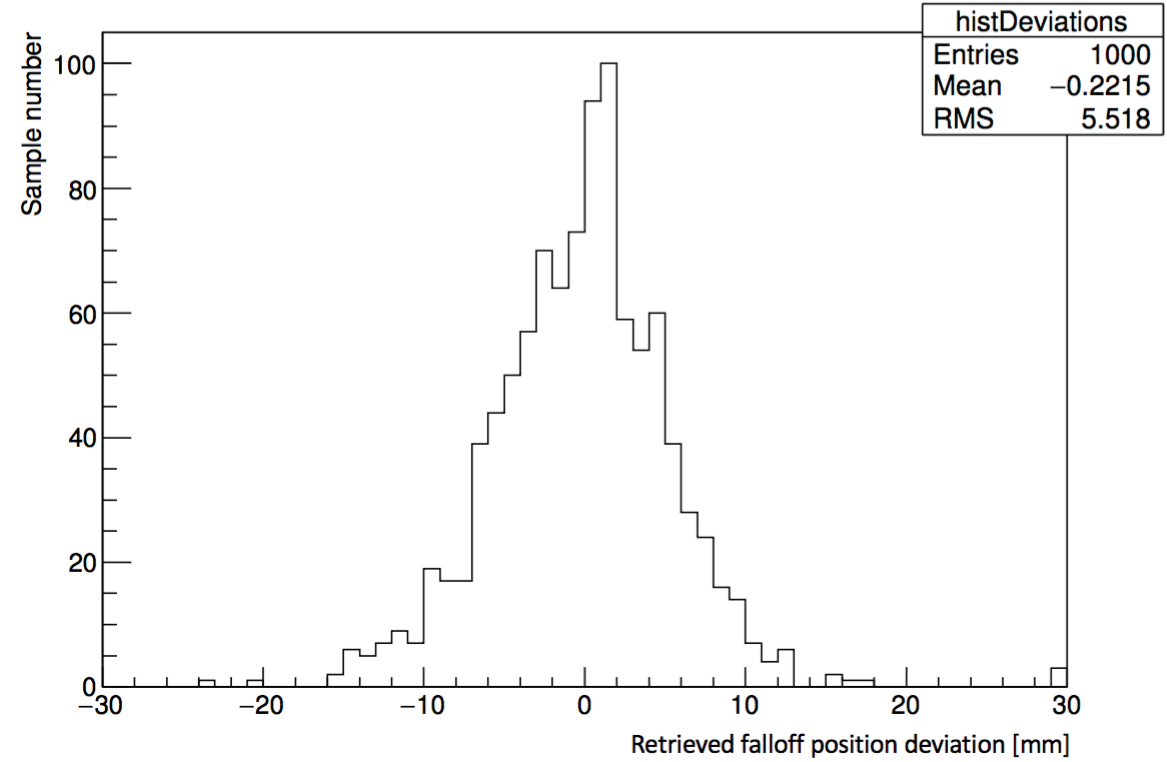
\includegraphics[width=0.48\textwidth]{./Figure/deviation_linecone.png}}
  % \subfloat[\label{fig:fig_Results_Precision_Distribution_Variation_CC_simulation_Hadronth_MLEM} ]{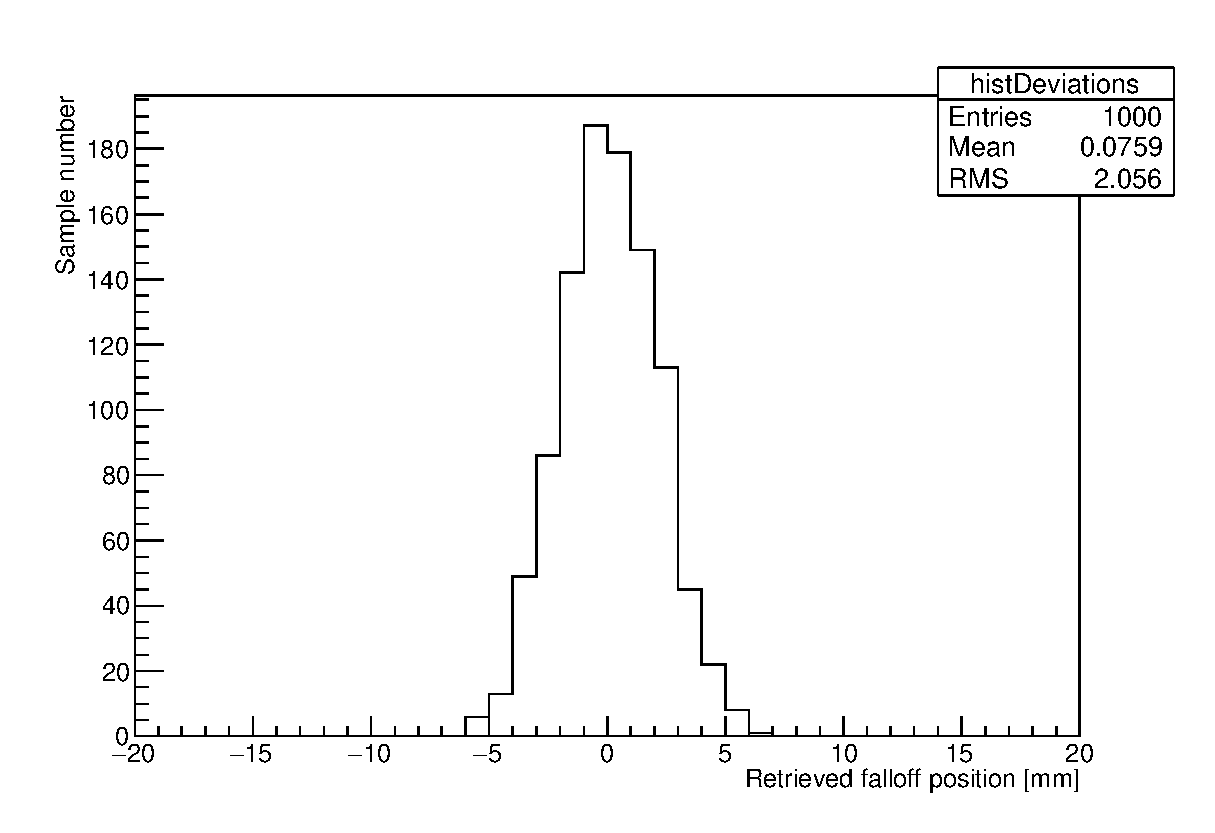
\includegraphics[width=0.33\textwidth]{./Figure/2017-08-02_FallOff_Results_binning_1mm_ShiftNurbs0_1mm_1e8_Article_MLEM.eps}}
  \subfloat[\label{fig:fig_Results_Precision_Distribution_Variation_CC_simulation_Hadronth_MLEM} ]{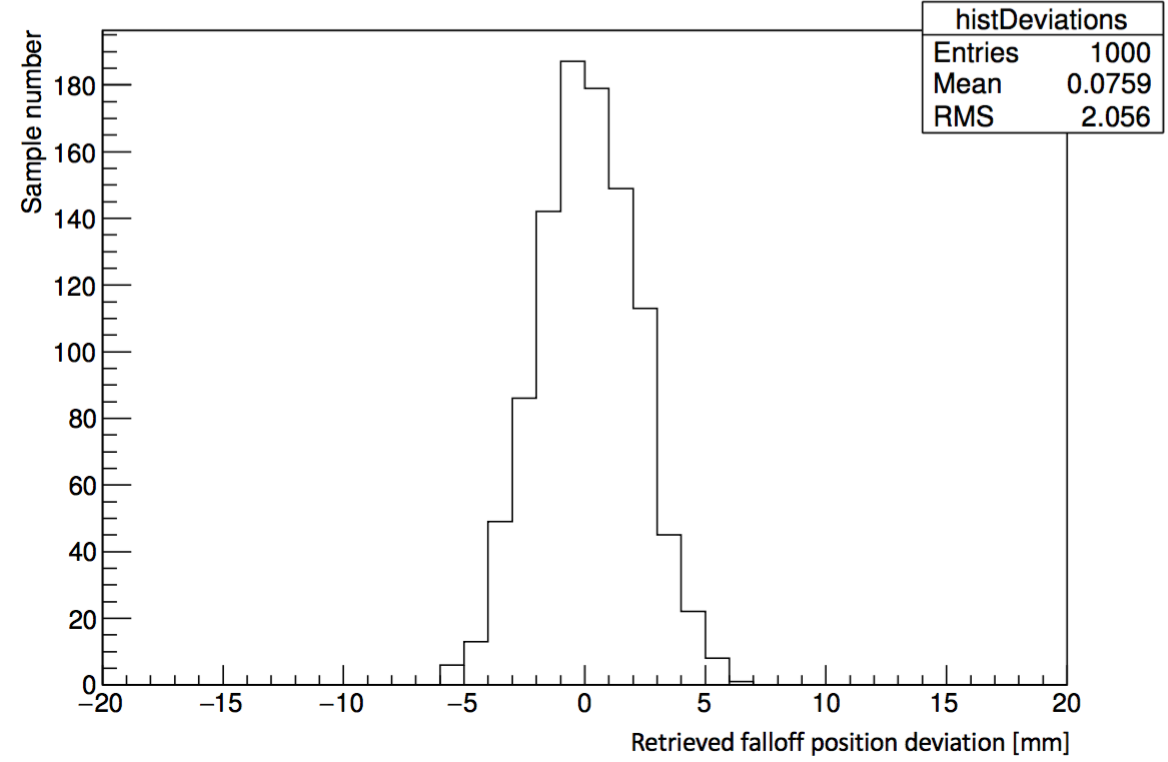
\includegraphics[width=0.48\textwidth]{./Figure/deviation_MLEM.png}}
  \caption{Data processing comparison for the same proton simulation with the line cone algorithm (left column) and the LM-MLEM algorithm (right column). The first row shows the $\chi^2$ distribution for one data subset. The last row represents the distribution of the minimal calculated shifts for 1000 such subsets.}% at the same statistics of $10^8$ incident protons.}
\end{figure}

\begin{figure}
\centering
\subfloat[]{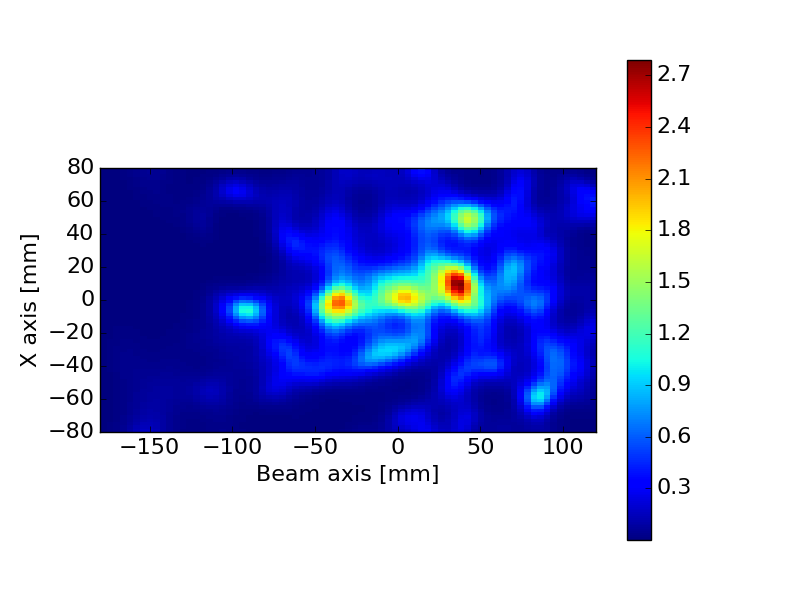
\includegraphics[width=0.5\textwidth,clip=true,trim=0 70 130 90]{./Figure/projection2D_Z_corr_r20.png}}
\subfloat[]{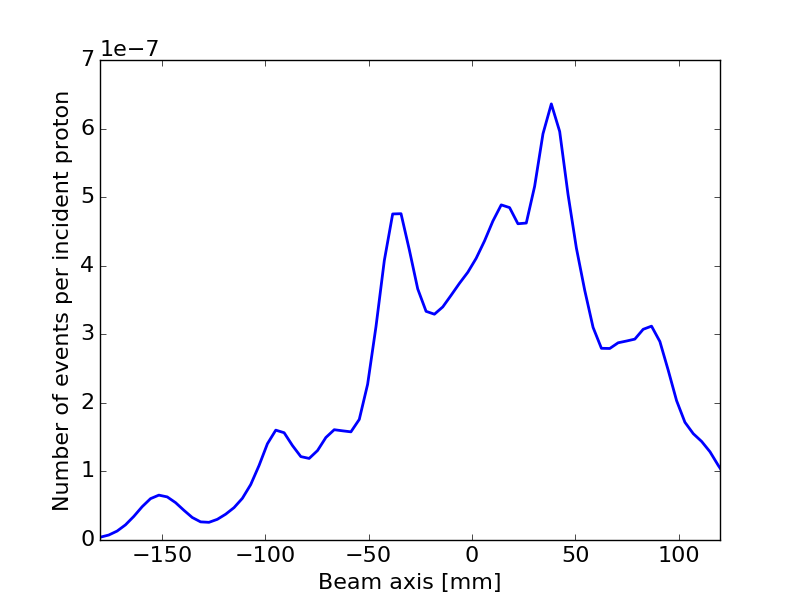
\includegraphics[width=0.5\textwidth]{./Figure/profileY_corr_r20.png}}\\
\subfloat[]{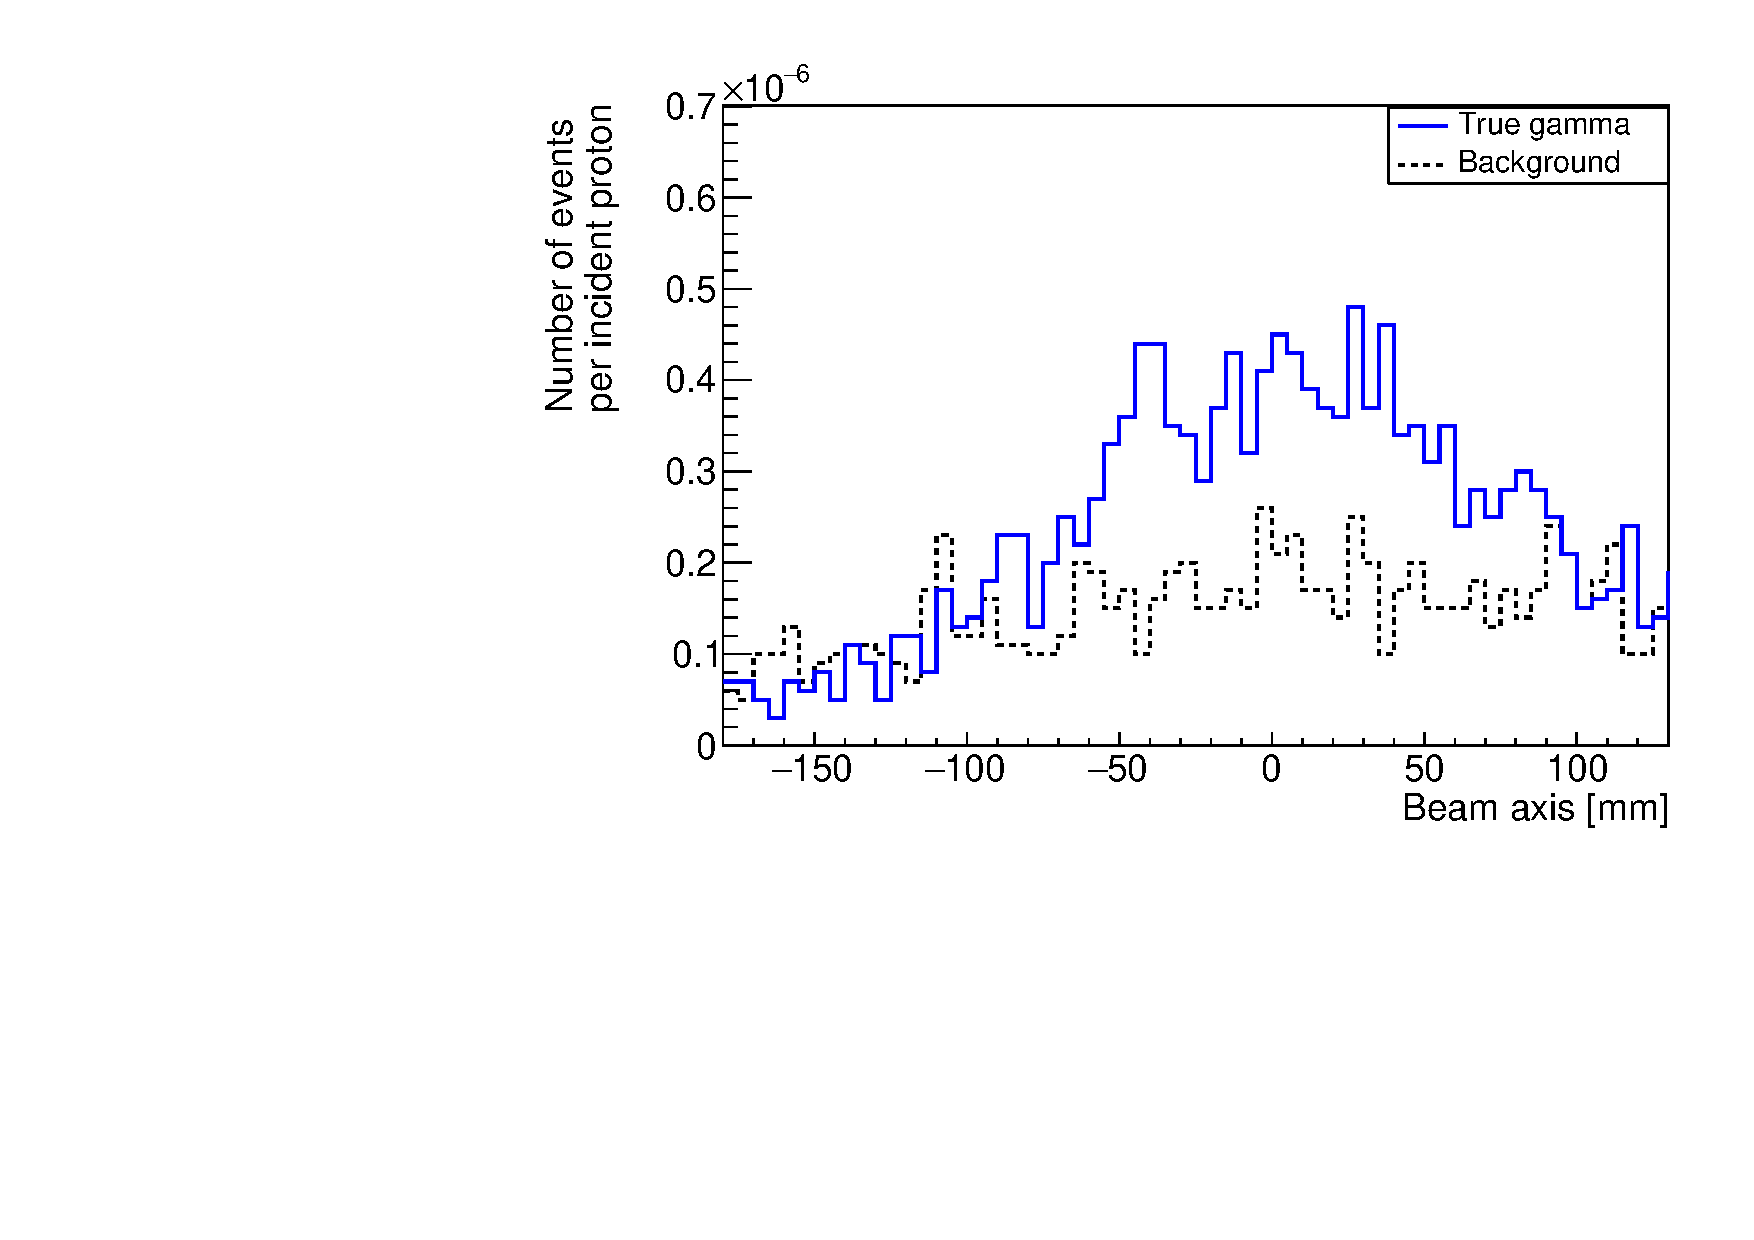
\includegraphics[width=0.5\textwidth]{./Figure/2015_02_16_Reconstruction_coinc_160MeVProton_TOF_6ns_file0to100_zoom.pdf}}
\caption{Line-cone and LM-MLEM reconstruction for a 160~MeV proton beam, $10^{8}$ total incident protons. The beam intensity is 1 proton per bunch. The Compton camera is centered at the expected Bragg peak position, $y=+50\,$mm. The time-of-flight event selection is applied on the collected data set. 20 iterations are performed for the MLEM reconstruction.
Figure (a) represents the MLEM reconstructed 2D image in the plane $(x,y)$, parallel to the camera entrance surface. The position $x=0\,$mm corresponds to the center of the PMMA phantom and the $y$ direction corresponds to the beam axis, with the target entrance at $y=-100\,$mm and the target end at $y=+100\,$mm.  In figure (b) the mono-dimensional profile along the $y$ axis is sketched. The profile fall-off is located at $y=+50\,$mm. Figure (c) shows the profile obtained by means of the line-cone algorithm for the same time-of-flight selected data.}
\label{fig:comparison}
\end{figure}


The analysis method described in section~\ref{MatMeth:precision} is applied to the different data set to retrieve the camera precision in the dose profile falloff identification. The results are shown in figure~\ref{fig:precision}, where the two reconstruction methods are represented by different markers.

\begin{figure}	
\centering
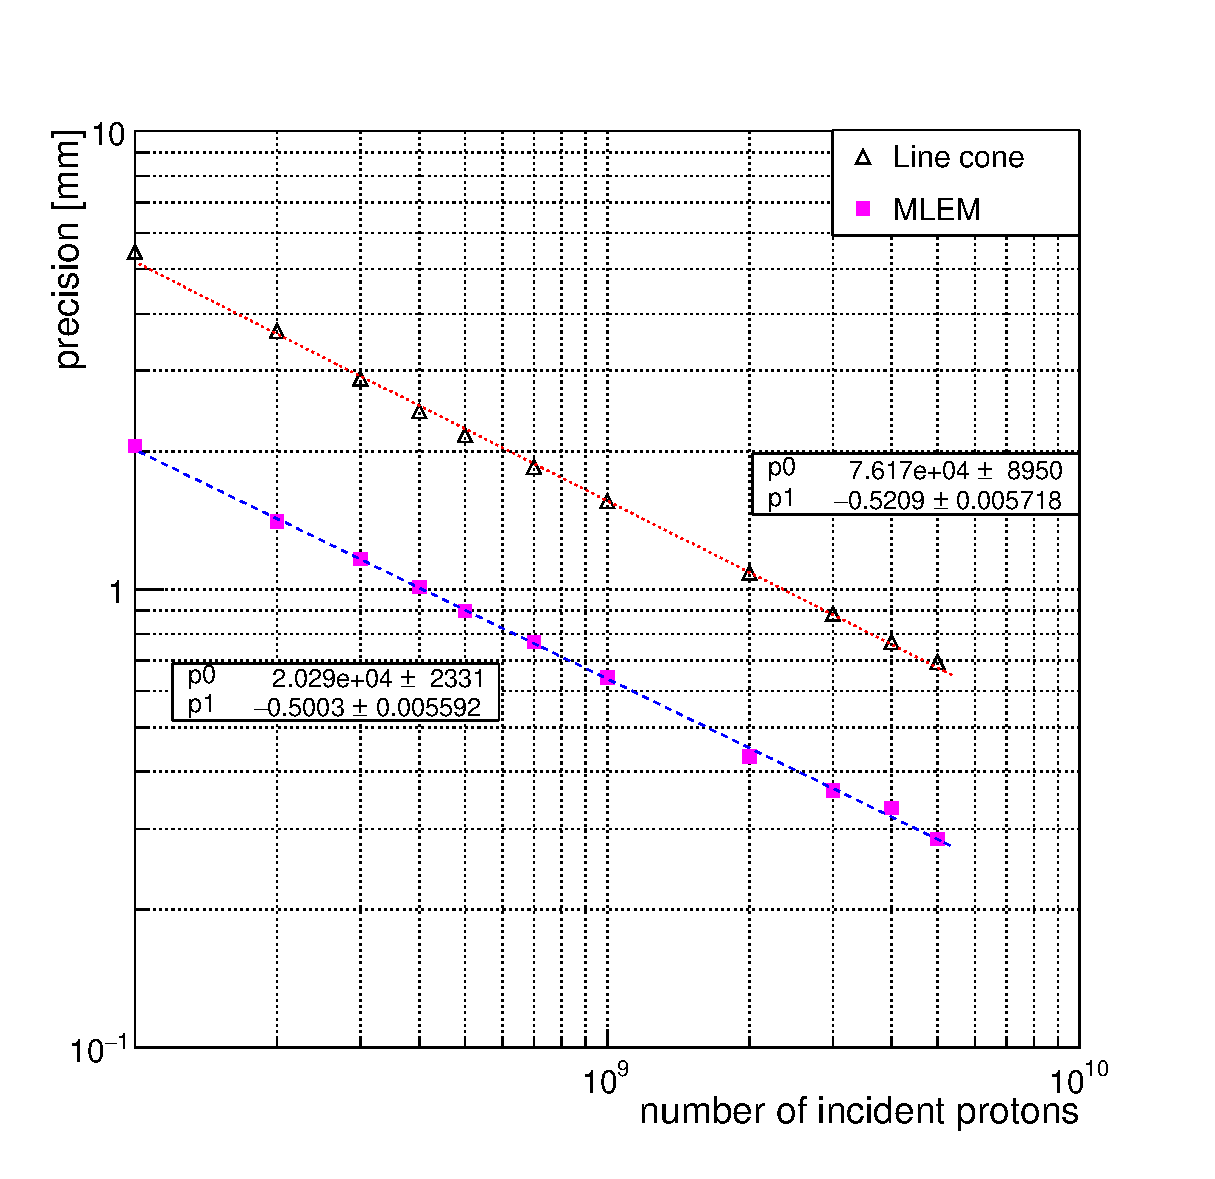
\includegraphics[width=0.7\textwidth]{./Figure/2017-10-21_Precision_Comparaison_linecone_MLEM_Article_Fit.eps}
\caption{Compton camera precision for two different reconstruction algorithms: line-cone and LM-MLEM. The precision is shown as a function of the total number of incident protons, in the range $1\times10^{8}$ to $5\times10^{9}$. A linear fit is realized on the results in order to obtain the slope of the results (p1 parameter in legend). A logarithmic scale is used on both axes. }	
\label{fig:precision}
\end{figure}

The iterative MLEM reconstruction method enables one to achieve a better precision, with a reduction of about 3~mm of the falloff retrieval accuracy in the whole range of statistics explored. A linear behavior, highlighted by the performed linear fit of the two data sets, is verified with increasing number of primary protons, starting from the single spot scale of about 10$^8$ primaries, till $5\times10^9$ protons, which can correspond to the monitoring of a group of spot with the same planned range. 

